%%__________________________________________________________________||
\section{Event selection}
\label{sec:event_selection}

The \alphat kinematic variable, first introduced in
Refs.~\cite{Randall:2008rw, RA1Paper}, is used to efficiently reject
events either without significant \met or with transverse energy
mismeasurements, while retaining sensitivity to new physics with
genuine \met signatures. The variable \alphat depends solely on the
measurements of the transverse energies and azimuthal angles of jets
and it is intrinsically robust against the presence of jet energy
mismeasurements in multijet systems.

For dijet events, the \alphat variable is defined as $\alphat =
\Et^{\rm j_2}/M_\text{T}$ where $\Et^{\rm j_2}$ is the transverse
energy of the less-energetic jet, and $M_\text{T}$ is the transverse
mass of the dijet system. 
For a perfectly measured dijet event with $\Et^{\mathrm{j}_1} =
\Et^{\mathrm{j}_2}$ and jets back-to-back in $\phi$, and in the limit
in which the momentum of each jet is large compared with its mass, the
value of \alphat is 0.5. For the case of an imbalance in the measured
transverse energies of back-to-back jets, \alphat is reduced to a
value smaller than 0.5, which gives the variable its intrinsic
robustness. % with respect to jet energy mismeasurements. 
%A similar behaviour is observed for energetic dijet events that
%contain neutrinos from the decay of a bottom or charm quark, as the
%neutrinos are typically collinear with respect to the axis of the
%heavy-flavour jet. 
Values significantly greater than 0.5 are observed when the two jets
are not back to back and are recoiling against significant, genuine
\met.

The definition of the \alphat variable can be generalised for events
with two or more jets. The mass scale of the physics processes being
probed is characterised by the scalar sum of the transverse energy
$\Et$ of jets considered in the analysis, defined as $\scalht =
\sum_{i=1}^{\njet} \Et^{\mathrm{j}_i}$, where \njet is the number of
jets with \Et above a predefined threshold. The estimator for \met is
given by the magnitude of the transverse momenta $\vec{\pt}$ vectorial
sum over these jets, defined as $\mht = |\sum_{i=1}^{N_\text{jet}}
\vec{\pt}^{\mathrm{j}_i}|$.  For events with three or more jets, a
pseudo-dijet system is formed by combining the jets in the event into
two pseudo-jets. The total \Et for each of the two pseudo-jets is
calculated as the scalar sum of the measured \Et of the contributing
jets. The combination chosen is the one that minimises the absolute
\Et difference between the two pseudo-jets, \dht. This simple
clustering criterion realises a balanced-event hypothesis and provides
the best separation between multijet events and events with genuine
\met. The \alphat definition can therefore be generalised as:

\begin{equation}
  \label{eq:alphat}
  \alphat = \frac{1}{2} \times \frac{\scalht -
    \dht}{\sqrt{\scalht^2 - \mht^2}}  = \frac{1}{2} \times
  \frac{1 - (\dht/\scalht)}{\sqrt{1 - (\mht/\scalht)^2}}\,. \nonumber
\end{equation}

In the presence of jet energy mismeasurements or neutrinos from
heavy-flavour quark decays, the direction and magnitude of the
apparent missing transverse energy, \mht, and energy imbalance of the
pseudo-dijet system, \dht, are highly correlated. This correlation is
much weaker for R-parity-conserving SUSY with each of the two decay
chains producing the LSP.

The event reconstruction and selection criteria described below are
explained in more detail in Ref.~\cite{RA1Paper2012}.
%Events containing non-collision backgrounds are suppressed by
%requiring at least one vertex of high-\pt tracks to be reconstructed
%in the luminous region. In the case of multiple vertices, the main
%interaction vertex is defined as the one with the highest scalar sum
%of ${\pt}^{2}$ of all associated tracks.
In order to suppress SM processes with genuine \met from neutrinos and
select only multijet final states, events containing an isolated
electron~\cite{PAS-EGM-10-004} or muon~\cite{PAS-MUO-10-004} with $\Pt
> 10\GeV$ or isolated photon~\cite{PAS-EGM-10-006} with $\pt > 25\GeV$
are vetoed. Furthermore, events containing an isolated
track~\cite{single-lepton-stop} with $\Pt > 10\gev$ are also vetoed.

Jets are reconstructed using the particle-flow (PF) reconstruction
algorithm~\cite{CMS-PAS-PFT-09-001, CMS-PAS-PFT-10-001} and 
clustered by the anti-$k_{\rm T}$ algorithm~\cite{antikt} with
a size parameter of $0.5$. The jet energies %measured by the
%calorimeter systems 
are corrected to account for the effects of pileup
and to establish a uniform relative response in $\eta$ and a
calibrated absolute response in transverse momentum
\pt~\cite{2011arXiv1107.4277C}.

Jets considered in the analysis are required to have a transverse
energy above $40\gev$ % thresholds summarised in
%Table~\ref{tab:thresholds}.  
%The two highest-$\Et$ jets are subjected
%to a higher \Et threshold and the highest-$\Et$ jet is required to be
%within the central tracker acceptance. 
Significant hadronic activity
in the event is ensured by requiring $\scalht > 200\GeV$ that also
ensures high efficiency for the trigger conditions, described below,
that record the event sample.
%  Lower jet \Et thresholds are employed
%for the region $200 < \scalht < 375\gev$ in order to maintain a
%background composition similar to that observed for the higher \scalht
%bins and to increase the analysis acceptance for SUSY models
%characterised by compressed mass spectra.
%
Events are vetoed if rare, spurious signals are identified in the
calorimeters~\cite{1748-0221-5-03-T03014, CMS-NOTE-2010-012} or if any
additional jet satisfies $\Et > 40\GeV$ and $|\eta| > 3$, in order to
maintain the performance of the variable \mht as an estimator of \met.

%\begin{table}[h!]
%  \caption{Thresholds on jet \Et, \scalht, and \alphat.\label{tab:thresholds}}
%  \centering
  %\footnotesize
%  \begin{tabular}{ lcccc }
%    \hline
%    \hline
%    \scalht (GeV)        & 200--275      & 275--325      & 325--375      & $>$375        \\
%    \hline
%    Jet \Et (GeV)        & 36.7          & 36.7          & 43.3          & 50.0          \\
%    Lead jet \Et (GeV)   & 73.3          & 73.3          & 86.7          & 100.0         \\
%    Second jet \Et (GeV) & 73.3          & 73.3          & 86.7          & 100.0         \\
%    \alphat              & 0.65          & 0.60          & 0.55          & 0.55          \\
%    \mht/\scalht        & $\gtrsim$0.64 & $\gtrsim$0.55 & $\gtrsim$0.42 & $\gtrsim$0.42 \\
%    \mht (GeV)          & $\gtrsim$130  & $\gtrsim$150  & $\gtrsim$135  & $\gtrsim$155  \\
%    \hline
%    \hline
%  \end{tabular}
%\end{table}

Events are categorised according to the number of jets per event,
%\njetlow or \njethigh, 
and the number of reconstructed b-quark jets
per event. For events with one jet (monojet events) the leading jet is required to have $\et > 200\gev$. Dijet events are split into two categories: symmetric, where the jets are both required to satisfy the same $100\gev$ \et threshold and asymmetric, where only the leading jet must satisfy $\et > 100\gev$. The motivation for these categories is improved sensitivity to direct pair-production of DM particles, where the analysis relies on the presence of jets from initial-state radiation. In addition, to improve sensitivity to new physics signals the \mht distrbution of the events is included as a discriminant in the analysis. A minimum bin width of $50\gev$ is chosen to minimise the number of events migrating between bins due to resolution effects, and a dedicated study is employed to assign a systematic uncertainity to the SM predictions in the \mht dimension.

%, $\nb = 0$, 1, 2, 3, or $\geq$4. 
%Eight (\njet,\nb) categories of events are considered in this
%analysis.
%For events containing exactly zero or one b-quark jets, eleven bins in
%\scalht are employed: three bins at low hadronic activity in the range
%$200 < \scalht < 375\gev$ as detailed in Table~\ref{tab:thresholds},
%plus an additional seven bins of width $100\gev$ in the range $375 <
%\scalht < 1075\gev$ and a final open bin $\scalht > 1075\gev$. For
%events containing exactly two or three (at least four) b-quark jets, a
%total of nine (four) bins in \scalht are used with a final open bin
%$\scalht > 875\gev$ ($\scalht > 375\gev$). This categorisation
%according to \njet, \nb, and \scalht results a total of 84 bins in the
%signal region.

For events satisfying the selection criteria described above, the
multijet background dominates over all other SM backgrounds. Multijet
events populate the region $\alphat \lesssim 0.5$ and the \alphat
distribution is characterised by a sharp edge at 0.5, beyond which the
multijet event yield falls by several orders of magnitude. \FIXMET{\alphat distn. figure goes here!}
Multijet events with extremely rare but large stochastic fluctuations in the
calorimetric measurements of jet energies can lead to values of
\alphat slightly above 0.5. The edge at 0.5 sharpens with increasing
\scalht for multijet events, primarily due to a corresponding increase
in the average jet energy and thus an improvement in the jet energy
resolution. This motivates a \scalt dependent \alphat requirement. \FIXME{Table of \alphat values per bin goes here}.

%The contribution from multijet events is suppressed by
%many orders of magnitude by requiring $\alphat > 0.55$

A number of beam- and detector-related effects can lead to events with
values of \alphat greater than 0.55, such as beam halo, reconstruction
failures, spurious detector noise, or event misreconstruction due to
detector inefficiencies. These events, with large, non-physical values
of \met, are rejected with high efficiency by applying a range of
dedicated vetoes~\cite{RA1Paper2012, cms-met}.

Two final, dedicated event vetoes complete the definition of the
hadronic signal region. The first veto concerns the rare circumstance
in which several jets with transverse energies below the \Et
thresholds and collinear in $\phi$ can result in significant \mht
relative to \met, the latter of which is less sensitive to jet \Et
thresholds and is determined by the particle-flow (PF) reconstruction
algorithm~\cite{CMS-PAS-PFT-09-001, CMS-PAS-PFT-10-001}. This type of
background, typical of multijet events, is suppressed while
maintaining high efficiency for SM or new physics processes with
genuine, significant \met by requiring $\mht / \met < 1.25$. 
%This
%behaviour is also utilised by the method to estimate the multijet
%background contamination per signal region bin, described below.

The second veto considers the minimum azimuthal angular separation of
a jet and the \mht vector derived from all other jets in the event,
known as \dphi~\cite{RA1Paper}. This variable is employed to suppress
any potential contribution from energetic multijet events that can
yield significant \met due to the production of neutrinos in
semileptonic heavy-flavour decays. The neutrinos are typically
collinear with respect to the axis of a jet and the requirement $\dphi
> 0.5$ has been demonstrated with data control samples to suppress
effectively this background source.

%As can be seen in Fig.~\ref{fig:aT}, the only expected remaining
%backgrounds with $\alpha_{\text{T}} > 0.55$ stem from SM processes
%with genuine \met in the final state. In the dijet case, the largest
%backgrounds with genuine \met are the associated production of W or Z
%bosons with jets, followed by either the weak decays \znunu or
%\wtaunu, where the $\tau$ decays hadronically and is identified as a
%jet; or by leptonic decays that are not rejected by the dedicated
%electron or muon vetoes. At higher jet multiplicities, top quark
%production, followed by semileptonic weak top quark decay, becomes
%important.

%\begin{figure}[bht]
%  \begin{center} 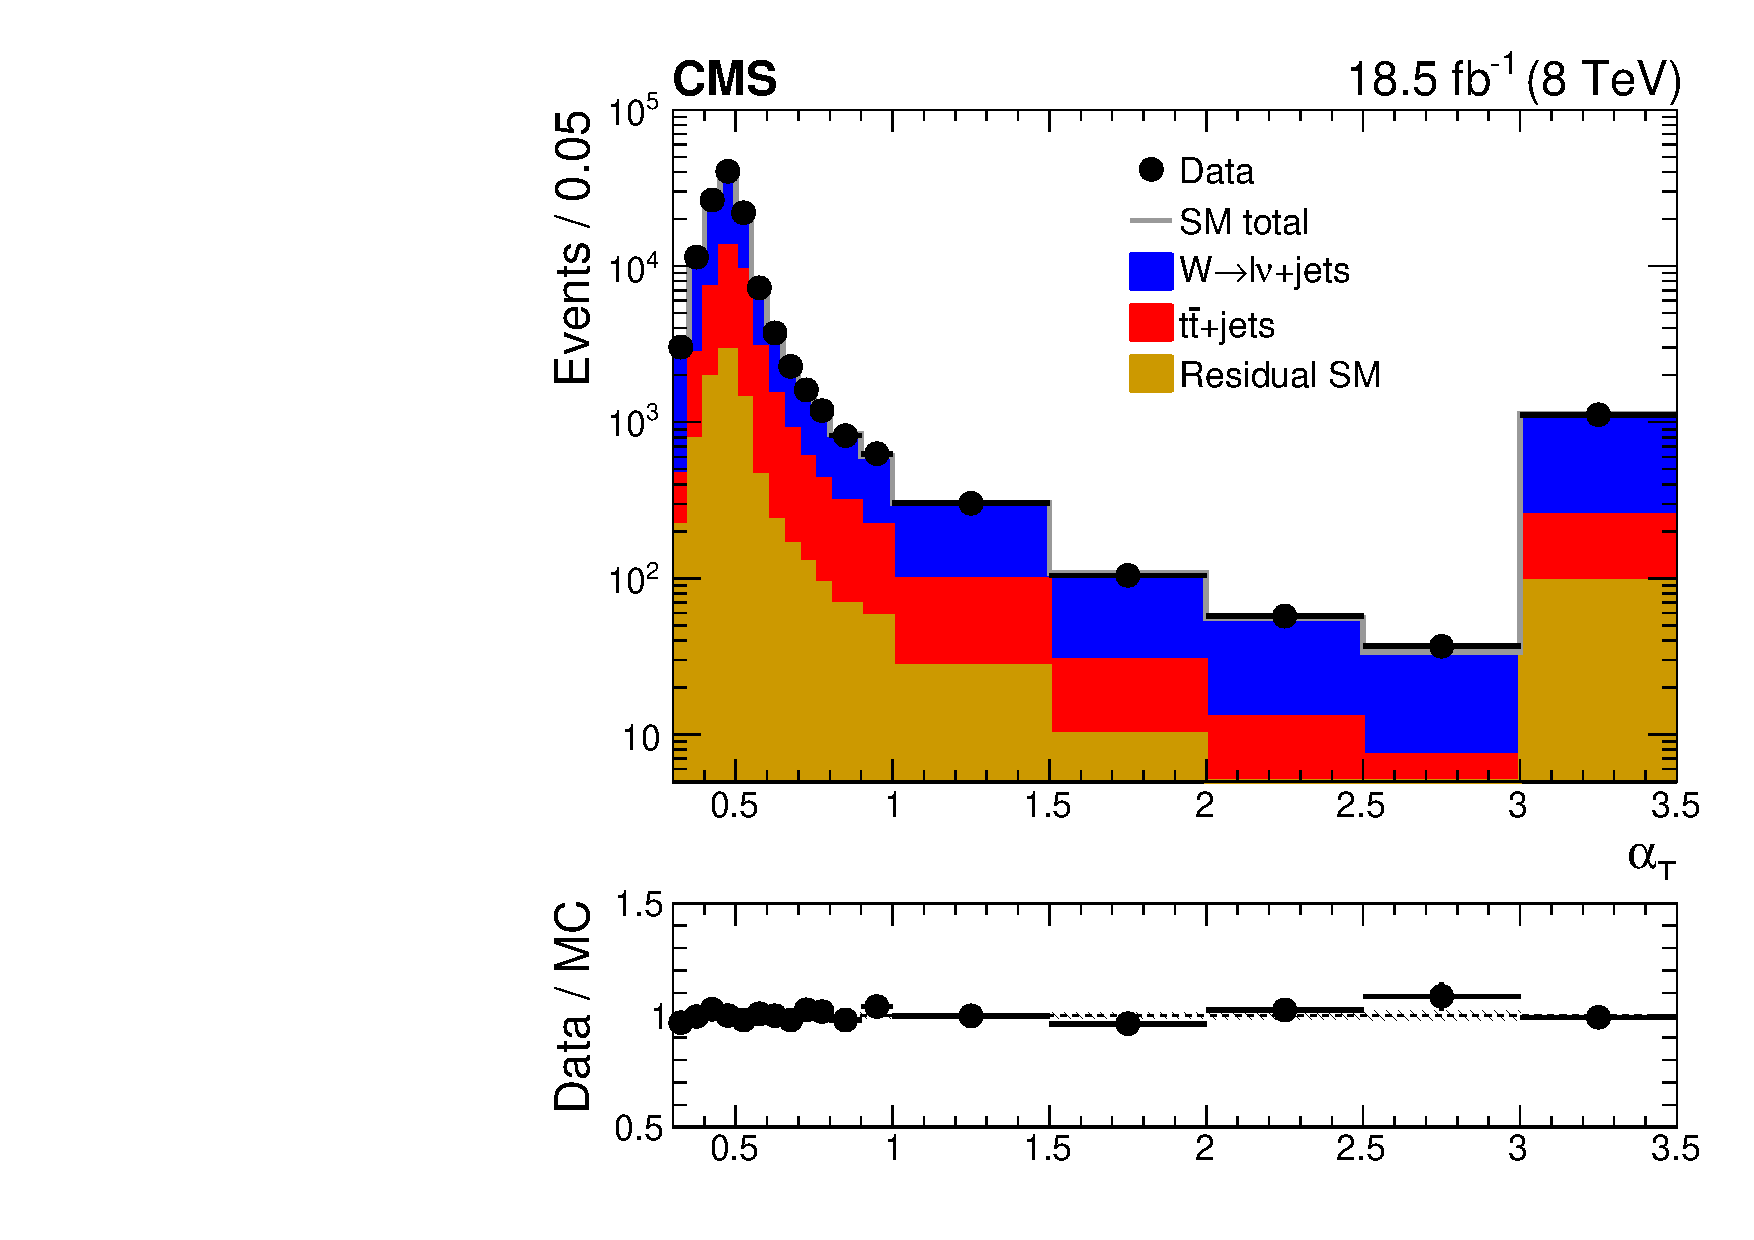
\includegraphics[width = \figwid]{AlphaT}
%    \caption{\label{fig:aT} The distribution of $\alpha_{\text{T}}$,
%      described in the text, for events in data with two or more jets
%      (black dots with error bars representing the statistical
%      uncertainties), after all event selection criteria except
%      $\alpha_{\text{T}}$ are applied and $\scalht > 375\GeV$. For
%      illustrative purposes only, expected yields from simulation are
%      also shown for QCD multi-jet events (dotted-dashed line),
%      associated production of top quarks, W, or Z with jets
%      (long-dashed line), the sum of all aforementioned SM processes
%      (solid line) and the SUSY LM6 model (dotted line). The
%      uncertainties for the SM expectation, due to the limited
%      accuracy of the available simulation datasets and jet energy
%      calibrations, are represented by the hatched area. The highest
%      bin contains the overflows.}
%    \end{center}
%\end{figure}

Signal candidate events are recorded with multiple jet-based trigger
conditions that require both \scalht and \alphat to satisfy
predetermined thresholds. The trigger-level jet energies are corrected
to account for energy scale and pileup effects. Different trigger
conditions are used depending on the \scalht bin and their
efficiencies are measured from data for each \njet category and
\scalht bin. Above \scalht of $800\gev$ no \alphat condition is applied. For monojet events a dedicated trigger based on a jet and missing energy condition is used.

%, which lie in the range 79--98\% ($>99\%$) for the region
%$200 < \scalht < 375\gev$ ($\scalht > 375\gev$). The non-negligible
%inefficiencies at low values of \scalht, which are accounted for in
%the final result, arise from conditions imposed on L1 trigger
%quantities.

%A set of prescaled $\scalht$ trigger conditions are used to record
%events for a hadronic control sample, which is defined by inverting
%either the \alphat and/or the \mhtmet requirements for the signal
%region. This event sample is used to estimate the multijet
%background contribution. 

Three disjoint data control regions, binned identically to the signal
region, are used to estimate the contributions from the various
remaining SM background processes. The control regions are defined by
a selection of \mj, \mmj, and \gj events. The selection criteria are
chosen such that the SM processes and their kinematic properties
resemble as closely as possible the SM background behaviour in the
signal region once the muon, dimuon system, or photon are ignored when
computing quantities such as \scalht and \alphat. 
%The event selection criteria are defined to ensure that any potential
%contamination from multijet events is negligible and also to suppress
%contributions from a wide variety of SUSY models (signal
%contamination) to a negligible level.
The event selection criteria are defined to ensure that any potential
contamination from multijet events or a wide variety of SUSY models
(\ie signal contamination) is negligible.

The \mj sample is recorded using a trigger condition that requires an
isolated muon and the event selection criteria are chosen in order for
the trigger to be maximally efficient at $\sim$90\%. Furthermore, the
muon is required to be well separated from the jets in the event and
the transverse mass ($M_{\rm T}$) of the muon and
\met~\cite{CMS-PAS-PFT-09-001, CMS-PAS-PFT-10-001} system must satisfy
$30 < M_{\rm T} < 125\gev$ to ensure a sample rich in W bosons
(produced promptly or from the decay of top quarks). The \mmj sample
uses similar selection criteria as the \mj sample and the same trigger
condition that yields an efficiency of $\sim$99\%. Exactly two
oppositely-charged, isolated muons are required, the muons must be
distanced from the jets in the event, and the invariant mass of the
dimuon system must be within a window of $\pm 25\GeV$ around the mass
of the Z boson. For both the muon and dimuon samples, no requirement
is made on the variable \alphat in order to increase the statistical
precision of the predictions derived from these samples.  The \gj
sample is recorded using a single photon trigger condition. The event
selection criteria comprise an isolated photon with $\Et > 200\gev$ and
$\scalht > 400\GeV$.%, and $\alphat > 0.55$, in order for the trigger to
%be maximally efficient at $\gtrsim$99\%.

\FIXME{Include \mht distrbutions figure for most important categories for gluino models}.

%%__________________________________________________________________||
